\documentclass[12pt,letterpaper]{article}
\usepackage[framemethod=tikz]{mdframed}
\usepackage[utf8]{inputenc} %Spanish input
\usepackage[T1]{fontenc} % Use 8-bit encoding that has 256 glyphs
\usepackage[spanish, es-tabla]{babel} % Selecciona el español para palabras introducidas automáticamente, p.ej. "septiembre" en la fecha y especifica que se use la palabra Tabla en vez de Cuadro
\usepackage{fullpage}
\usepackage[top=2cm, bottom=4.5cm, left=2.5cm, right=2.5cm]{geometry}
\usepackage{lastpage}
\usepackage{enumerate}
\usepackage[inline]{enumitem}
\usepackage{fancyhdr}
\usepackage{xcolor}
\usepackage{listings}
%
\usepackage[sorting=none]{biblatex}
\addbibresource{citas.bib}
%
\usepackage{csquotes}
\usepackage{cellspace}
\setlength{\cellspacetoplimit}{5pt}
\setlength{\cellspacebottomlimit}{5pt}
\usepackage{hhline}
\usepackage{listings}
\usepackage{hyperref}
\usepackage{titletoc,tocloft}
\usepackage{float,subfig}
\setlength{\cftsubsecindent}{2cm}
\setlength{\cftsubsubsecindent}{4cm}
\dottedcontents{section}[1.5em]{}{1.3em}{.6em}
%\usepackage[nodisplayskipstretch]{setspace}
%
\graphicspath{ {./imgs/} } %Drawing the background pic
\usepackage{tikz}
\newcommand{\tikzmark}[1]{\tikz[baseline,remember picture] \coordinate (#1) {};}
\usetikzlibrary{positioning}
\usetikzlibrary{shadows,arrows.meta} % For adding edges label
\usetikzlibrary{calc}
\usepackage{eso-pic}
\AddToShipoutPictureBG{%
    \begin{tikzpicture}[remember picture, overlay]
        \node[opacity=.15, inner sep=0pt]
            at(current page.center){
\includegraphics[scale=1.5]{logo-ugr2}};
    \end{tikzpicture}%
}

% \numberwithin{equation}{section} % Number equations within sections (i.e. 1.1, 1.2, 2.1, 2.2 instead of 1, 2, 3, 4)
% \numberwithin{figure}{section} % Number figures within sections (i.e. 1.1, 1.2, 2.1, 2.2 instead of 1, 2, 3, 4)
% \numberwithin{table}{section} % Number tables within sections (i.e. 1.1, 1.2, 2.1, 2.2 instead of 1, 2, 3, 4)

\hypersetup{%
    colorlinks=true,
    linkcolor=[rgb]{0.2, 0.3, 0.5},
    urlcolor=black,
    citecolor=black,
    linkbordercolor={0 0 1}
}

\renewcommand\lstlistingname{Código:}
\renewcommand\lstlistlistingname{Código:}
\def\lstlistingautorefname{Brian SS.}
%
%
\newcommand{\horrule}[1]{\rule{\linewidth}{#1}} % Create horizontal rule command with 1 argument of height
\definecolor{codegreen}{rgb}{0,0.6,0}
\definecolor{codegray}{rgb}{0.5,0.5,0.5}
\definecolor{codepurple}{rgb}{0.58,0,0.82}
\definecolor{backcolour}{rgb}{0.95,0.95,0.92}
%
\lstset{language=python,basicstyle=\linespread{1.1}\ttfamily\footnotesize,
    xleftmargin=0.0cm, frame=t, framesep=0.15cm, framerule=0pt, tabsize=4,
    showspaces=false, showstringspaces=false,showlines=true,
    keywordstyle=\color{blue}\ttfamily,
    stringstyle=\color{red}\ttfamily,
    commentstyle=\color{gray}\ttfamily,
    morecomment=[l][\color{magenta}]{\#}
}
%
\setlength{\parindent}{0.0in}
\setlength{\parskip}{0.05in}
%
%% Edit these as appropriate
\newcommand\course{Ciencia de Datos e Ingenieria de Computadores}
\newcommand\hwnumber{1}                  % <-- homework number
\newcommand\NetIDa{}           % <-- NetID of person #1
\newcommand\NetIDb{}           % <-- NetID of person #1
%
\pagestyle{fancyplain}
\headheight 35pt
\lhead{\NetIDa}
%\lhead{\NetIDa\\\NetIDb}                 % <-- Comment this line out for problem sets (make sure you are person #1)
\lhead{\textbf{\large Preprocesamiento y Clasificación}}
\rhead{\course \\ \today}
\lfoot{\scriptsize\LaTeX}
\cfoot{\hyperlink{Indice}{Volver al índice}}
\rfoot{\small\thepage}
\headsep 1.5em
%
\renewcommand*\contentsname{Índice}
%
\author{Brian Sena Simons} % Nombre y apellidos
%
\date{\normalsize\today} % Incluye la fecha actual
%
\begin{document}
%
\begin{titlepage}
\begin{figure}[H]
    \vspace{-1.3cm}
    \begin{center}
        
\includegraphics[width=0.75\textwidth]{Etsiit}
    \end{center}
\end{figure}
\vspace{1.3cm}
\centering
\normalfont \normalsize
\textsc{\textbf{Minería de Datos} \\ \vspace{.15cm} Master en Ciencia de Datos e Ingeniería de Computadores \\ \vspace{.15cm} Universidad de Granada} \\ [25pt] % Your university, school and/or department name(s)
    \horrule{0.5pt} \\[0.4cm] % Thin top horizontal rule
    \huge Preprocesamiento y Clasificación\\ % The assignment title
    \horrule{2pt} \\[0.5cm] % Thick bottom horizontal rule

\begin{minipage}{0.4\textwidth}
    \begin{flushleft}\large
        \emph{Autores:} \\
         ----------------------- \\
        \vspace{.15cm}
        Brian Sena Simons. \\
        Miguel Garcia Lopez. \\
        Álvaro Santana Sánchez. \\ 
        Ana Fuentes Rodríguez.

    \end{flushleft}
\end{minipage}
\begin{minipage}{0.4\textwidth}
    \vspace{-2.2cm}
     \begin{flushright}\large
         Grupo: \\
         ----------------------- \\
         Data Mavericks.
    \end{flushright}
\end{minipage}
\end{titlepage}


\hypertarget{Indice}{}
\tableofcontents
\newpage
\section{Introducción.}
Se ha realizado un análisis y comparativa entre diferentes modelos para la detección de anomalías y predicción de vida útil restante (RUL por sus siglas en inglés)
en compresores del sector ferroviario. Para ello, se ha utilizado el conjunto de datos (dataset) ``MetroPT-3''~\cite{MetroPT-3}.
Está publicado en ``UCI Machine Learning Repository''~\cite{UCIMLR} y, según la descripción, MetroPT-3~\cite{MetroPT-3} es un conjunto de datos multivariantes de series temporales. Los datos provienen de sensores analógicos y digitales 
instalados en un compresor de tren, que miden 15 señales como presiones, corriente del motor, temperatura del aceite y señales eléctricas de las válvulas de entrada de aire. 
La información fue registrada a una frecuencia de 1 Hz entre febrero y agosto de 2020 (véase Tabla~\ref{tab:DatosBasicos})

\begin{table}[htp]
    \centering
    \begin{tabular}{|l|l|l|c|c|c|c|c|c|}
    \hline
        \textbf{Variable} & \textbf{Tipo} & \textbf{Mín.} & \textbf{Q1} & \textbf{Q2} & \textbf{Media} & \textbf{Q3} & \textbf{Máx.} \\ \hline
TP2               & Numérico      & -0.032        & -0.014      & -0.012      & 1.368         & -0.010      & 10.676        \\ \hline
TP3               & Numérico      & 0.730         & 8.492       & 8.960       & 8.985         & 9.492       & 10.302        \\ \hline
H1                & Numérico      & -0.036        & 8.254       & 8.784       & 7.568         & 9.374       & 10.288        \\ \hline
DV\_pressure      & Numérico      & -0.032        & -0.022      & -0.020      & 0.05596       & -0.018      & 9.844         \\ \hline
Reservoirs        & Numérico      & 0.712         & 8.494       & 8.960       & 8.985         & 9.492       & 10.300        \\ \hline
Oil\_temperature  & Numérico      & 15.40         & 57.77       & 62.70       & 62.64         & 67.25       & 89.05         \\ \hline
Motor\_current    & Numérico      & 0.020         & 0.040       & 0.045       & 2.050         & 3.808       & 9.295         \\ \hline
COMP              & Numérico      & 0.000         & 1.000       & 1.000       & 0.837         & 1.000       & 1.000         \\ \hline
DV\_eletric       & Numérico      & 0.000         & 0.000       & 0.000       & 0.1606        & 0.000       & 1.000         \\ \hline
Towers            & Numérico      & 0.000         & 1.000       & 1.000       & 0.9198        & 1.000       & 1.000         \\ \hline
MPG               & Numérico      & 0.000         & 1.000       & 1.000       & 0.8327        & 1.000       & 1.000         \\ \hline
LPS               & Numérico      & 0.000         & 0.000       & 0.000       & 0.00342       & 0.000       & 1.000         \\ \hline
Pressure\_switch  & Numérico      & 0.000         & 1.000       & 1.000       & 0.9914        & 1.000       & 1.000         \\ \hline
Oil\_level        & Numérico      & 0.000         & 1.000       & 1.000       & 0.9042        & 1.000       & 1.000         \\ \hline
Caudal\_impulses  & Numérico      & 0.000         & 1.000       & 1.000       & 0.9371        & 1.000       & 1.000         \\ \hline
    \end{tabular}
    \caption{Información básica de los diferentes tipos de datos presentes en MetroPT-3~\cite{MetroPT-3}}
    \label{tab:DatosBasicos}
\end{table}

Las variables que analógicas que observamos son:
\begin{enumerate}
    \item TP2 (bar): La medición de la presión en el compresor.
    \item TP3 (bar): La medición de la presión generada en el panel neumático.
    \item H1 (bar): La medición de la presión generada debido a la caída de presión cuando ocurre la descarga del filtro separador ciclónico.
    \item Presión DV (bar): La medición de la caída de presión generada cuando las torres descargan los secadores de aire; una lectura de cero indica que el compresor está operando bajo carga.
    \item Reservorios (bar): La medición de la presión aguas abajo de los reservorios, que debería ser cercana a la presión del panel neumático (TP3).
    \item Corriente del Motor (A): La medición de la corriente de una fase del motor trifásico; presenta valores cercanos a 0A (cuando está apagado), 4A (cuando trabaja sin carga), 7A (cuando trabaja bajo carga) y 9A (cuando empieza a trabajar).
    \item Temperatura del Aceite (ºC): La medición de la temperatura del aceite en el compresor.
\end{enumerate}
Las variables digitales que observamos son: 
\begin{enumerate}
    \item COMP: La señal de la válvula de admisión de aire del compresor; está activa cuando no hay admisión de aire, lo que indica que el compresor está apagado o funcionando sin carga.
    \item DV eléctrico: La señal que controla la válvula de salida del compresor; está activa cuando el compresor funciona bajo carga e inactiva cuando el compresor está apagado o funcionando sin carga.
    \item TORRES: La señal que define la torre responsable de secar el aire y la torre responsable de drenar la humedad eliminada del aire; cuando no está activa, indica que la torre uno está funcionando; cuando está activa, indica que la torre dos está en operación.
    \item MPG: La señal responsable de arrancar el compresor bajo carga activando la válvula de admisión cuando la presión en la unidad de producción de aire (APU) cae por debajo de 8.2 bar; activa el sensor COMP.
    \item LPS: La señal que detecta y activa cuando la presión cae por debajo de 7 bares.
    \item Interruptor de Presión: La señal que detecta la descarga en las torres de secado.
    \item Nivel de Aceite: La señal que detecta el nivel de aceite en el compresor; está activa cuando el nivel de aceite está por debajo de los valores esperados.
    \item Impulso de Caudal: La señal que cuenta los pulsos generados por la cantidad absoluta de aire que fluye desde la APU hacia los reservorios.
\end{enumerate}


Este conjunto de datos tiene como objetivo principal mejorar la detección de fallos y la predicción de mantenimiento. 
Aunque no contiene etiquetas directas, se dispone de informes de fallos que permiten evaluar la efectividad de los algoritmos de detección de anomalías, predicción de fallos y estimación de RUL (véase la Tabla~\ref{tab:Reportes}).

\begin{table}[htp]
    \centering
\begin{tabular}{|c|l|l|r|l|}
\hline
\textbf{Número} & \textbf{Inicio}       & \textbf{Fin}         & \textbf{Duración (mín)} & \textbf{Importancia} \\ \hline
1            & 4/12/2020 11:50          & 4/12/2020 23:30           & 700                & Alta              \\ \hline
2            & 4/18/2020 00:00          & 4/18/2020 23:59           & 1440               & Alta              \\ \hline
3            & 4/19/2020 00:00          & 4/19/2020 01:30           & 90                 & Alta              \\ \hline
4            & 4/29/2020 03:20          & 4/29/2020 04:00           & 40                 & Alta              \\ \hline
5            & 4/29/2020 22:00          & 4/29/2020 22:20           & 20                 & Alta              \\ \hline
6            & 5/13/2020 14:00          & 5/13/2020 23:59           & 599                & Alta              \\ \hline
7            & 5/18/2020 05:00          & 5/18/2020 05:30           & 30                 & Alta              \\ \hline
8            & 5/19/2020 10:10          & 5/19/2020 11:00           & 50                 & Alta              \\ \hline
9            & 5/19/2020 22:10          & 5/19/2020 23:59           & 109                & Alta              \\ \hline
10           & 5/20/2020 00:00          & 5/20/2020 20:00           & 1200               & Alta              \\ \hline
11           & 5/23/2020 09:50          & 5/23/2020 10:10           & 20                 & Alta              \\ \hline
12           & 5/29/2020 23:30          & 5/29/2020 23:59           & 29                 & Alta              \\ \hline
13           & 5/30/2020 00:00          & 5/30/2020 06:00           & 360                & Alta              \\ \hline
14           & 6/01/2020 15:00          & 6/01/2020 15:40           & 40                 & Alta              \\ \hline
15           & 6/03/2020 10:00          & 6/03/2020 11:00           & 60                 & Alta              \\ \hline
16           & 6/05/2020 10:00          & 6/05/2020 23:59           & 839                & Alta              \\ \hline
17           & 6/06/2020 00:00          & 6/06/2020 23:59           & 1439               & Alta              \\ \hline
18           & 6/07/2020 00:00          & 6/07/2020 14:30           & 870                & Alta              \\ \hline
19           & 7/08/2020 17:30          & 7/08/2020 19:00           & 90                 & Alta              \\ \hline
20           & 7/15/2020 14:30          & 7/15/2020 19:00           & 270                & Media            \\ \hline
21           & 7/17/2020 04:30          & 7/17/2020 05:30           & 60                 & Alta              \\ \hline
\end{tabular}
    \caption{
    Intervalos de tiempo con problemas en la compresión del aire.
    Nos permite evaluar la capacidad de detección anomalías de nuestros modelo.}
    \label{tab:Reportes}
\end{table}

Además, se recomienda utilizar el primer mes de datos para entrenar modelos, dejando el resto para las pruebas, permitiendo también la formación incremental si fuera necesario.


\section{Análisis Exploratorio de Datos.}
Se tienen más de un millón de observaciones correspondientes a distintos momentos en el tiempo que capturan datos de distintos sensores. Todas las variables son continuas a excepción del \textit{timestamp}, que es la fecha de registro de cada valor en las variables.
No hay nulos, por lo que no se requiere ningún tratamiento especial (como imputaciones) para ese tipo de casos. Lo que sí ocurre es que hay pequeños intervalos de tiempo vacíos, sin datos, pero estos no aparecen como nulos, solo pasa de un intervalo a otro en un salto temporal que se salta parte del tiempo. En ese caso se ha considerado válido eliminar ese espacio temporal por ser mínimo y por no tener información de si podría haber anomalía o no. Otra opción habría sido imputar ese espacio temporal con datos sintéticos que repliquen los datos del espacio temporal anterior, pero se consideró más válido eliminar ese intervalo.

\subsection{Transformaciones y Visualizaciones}
Se estandarizan los datos para poder visualizarlos y que las escalas no afecten demasiado a estas visualizaciones. No se normaliza por la desviación típica, ya que se desea conservar la variación de los datos. De esta forma no se pierde su relación original de escalas.

\begin{figure}[htp]
    \centering
    \begin{minipage}[b]{0.45\textwidth}
        \centering
        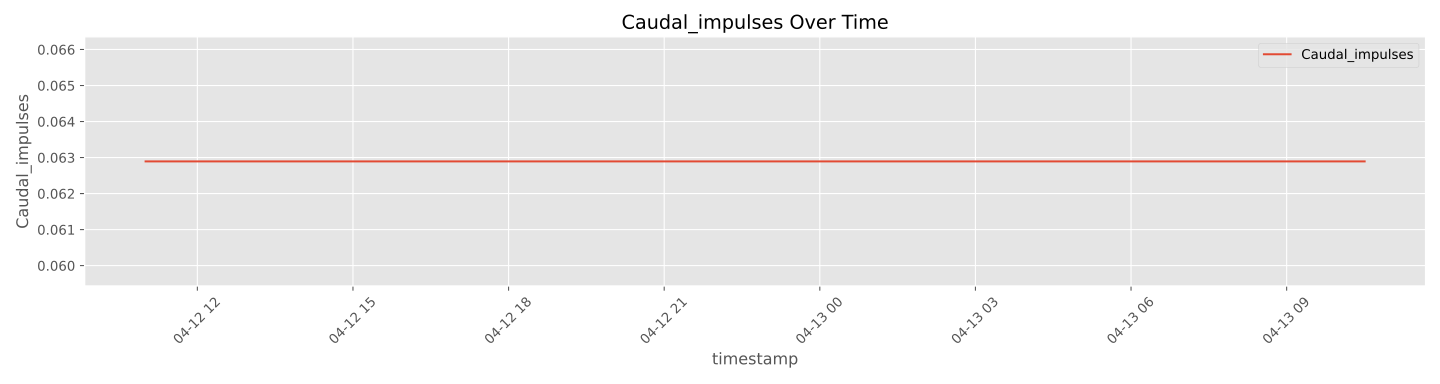
\includegraphics[width=\textwidth]{Caudal_impulses.png}
        \caption*{Caudal Impulses}
    \end{minipage}
    \hfill
    \begin{minipage}[b]{0.45\textwidth}
        \centering
        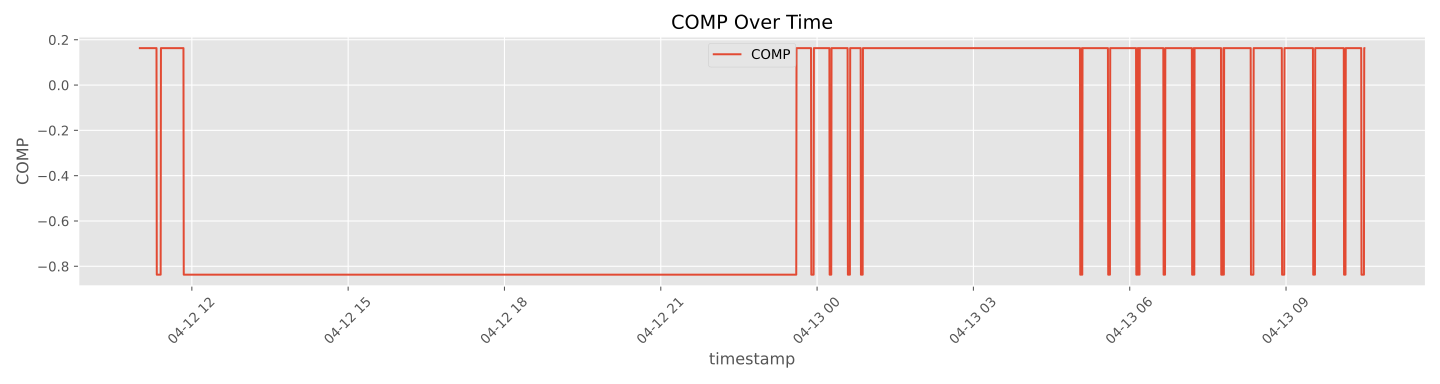
\includegraphics[width=\textwidth]{COMP.png}
        \caption*{COMP}
    \end{minipage}
    \vspace{0.5em} % Adds space between rows

    \begin{minipage}[b]{0.45\textwidth}
        \centering
        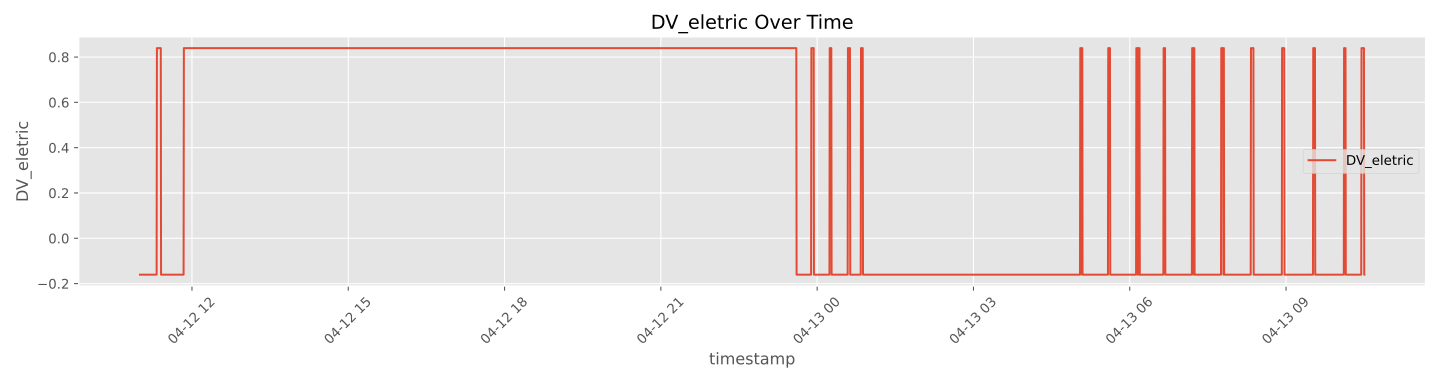
\includegraphics[width=\textwidth]{DV_eletric.png}
        \caption*{DV Electric}
    \end{minipage}
    \hfill
    \begin{minipage}[b]{0.45\textwidth}
        \centering
        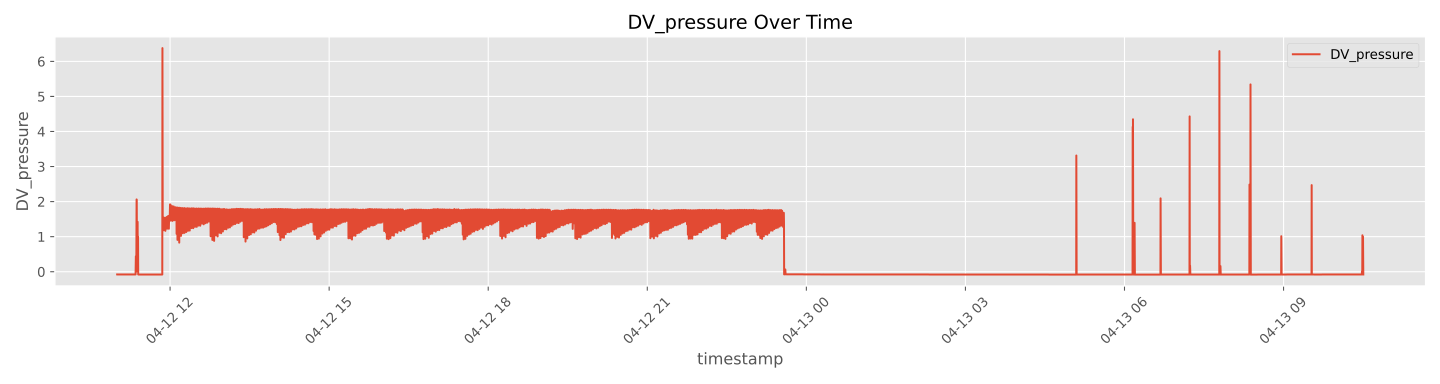
\includegraphics[width=\textwidth]{DV_pressure.png}
        \caption*{DV Pressure}
    \end{minipage}
    \vspace{0.5em}

    \begin{minipage}[b]{0.45\textwidth}
        \centering
        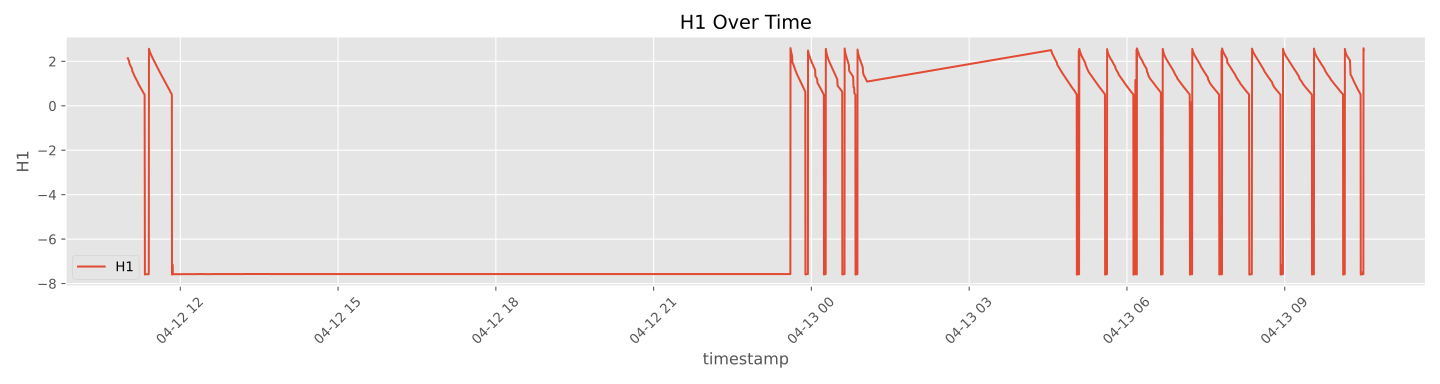
\includegraphics[width=\textwidth]{H1.png}
        \caption*{H1}
    \end{minipage}
    \hfill
    \begin{minipage}[b]{0.45\textwidth}
        \centering
        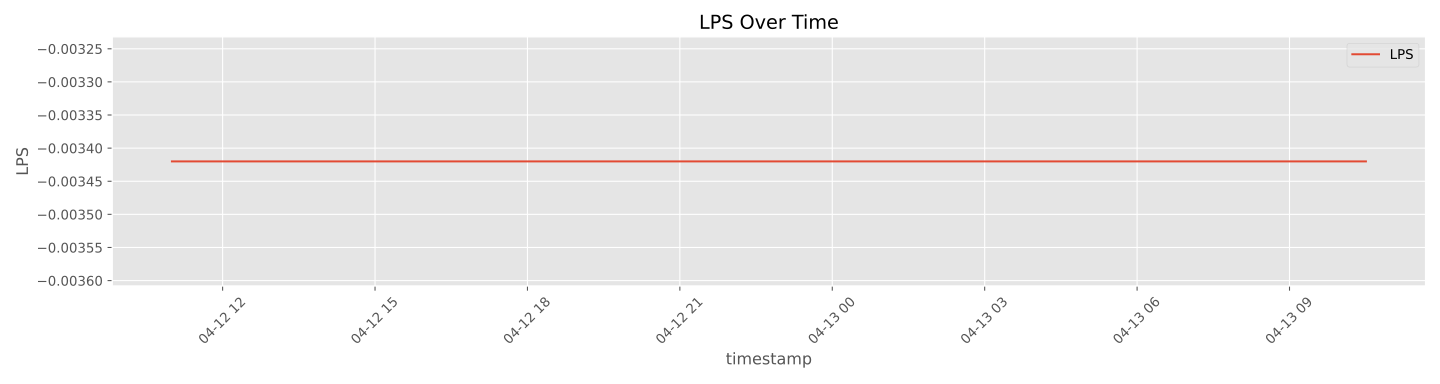
\includegraphics[width=\textwidth]{LPS.png}
        \caption*{LPS}
    \end{minipage}
    \vspace{0.5em}

    \begin{minipage}[b]{0.45\textwidth}
        \centering
        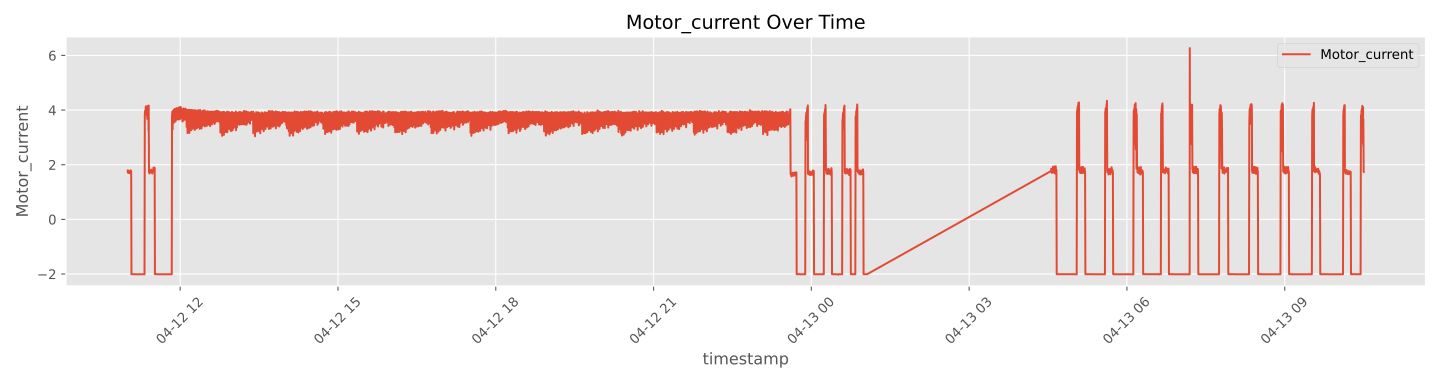
\includegraphics[width=\textwidth]{Motor_current.png}
        \caption*{Motor Current}
    \end{minipage}
    \hfill
    \begin{minipage}[b]{0.45\textwidth}
        \centering
        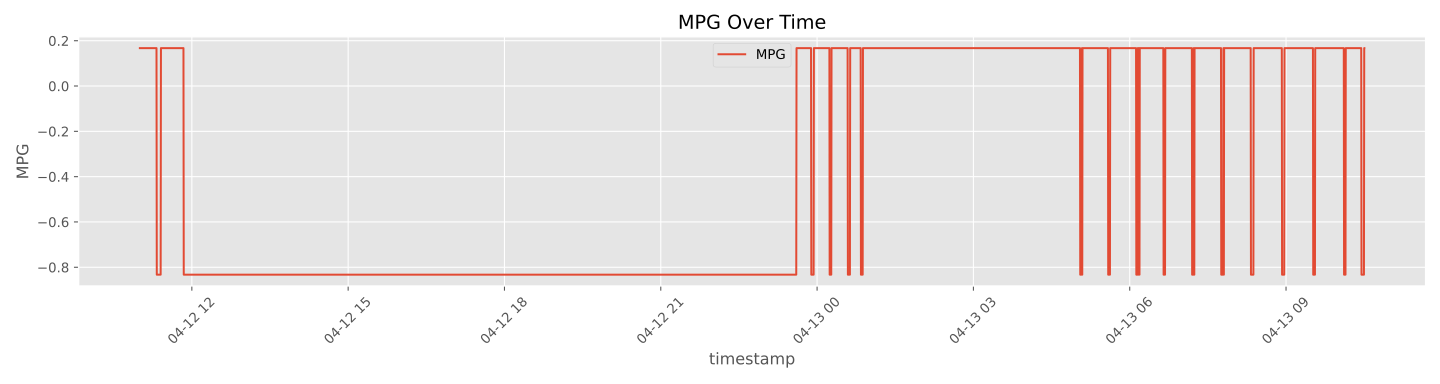
\includegraphics[width=\textwidth]{MPG.png}
        \caption*{MPG}
    \end{minipage}
    \vspace{0.5em}

    \begin{minipage}[b]{0.45\textwidth}
        \centering
        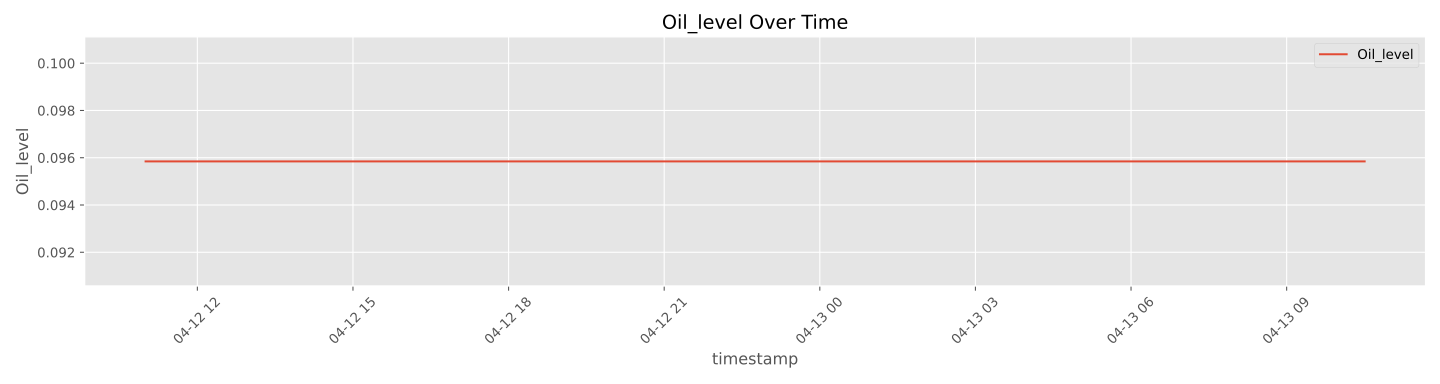
\includegraphics[width=\textwidth]{Oil_level.png}
        \caption*{Oil level}
    \end{minipage}
    \hfill
    \begin{minipage}[b]{0.45\textwidth}
        \centering
        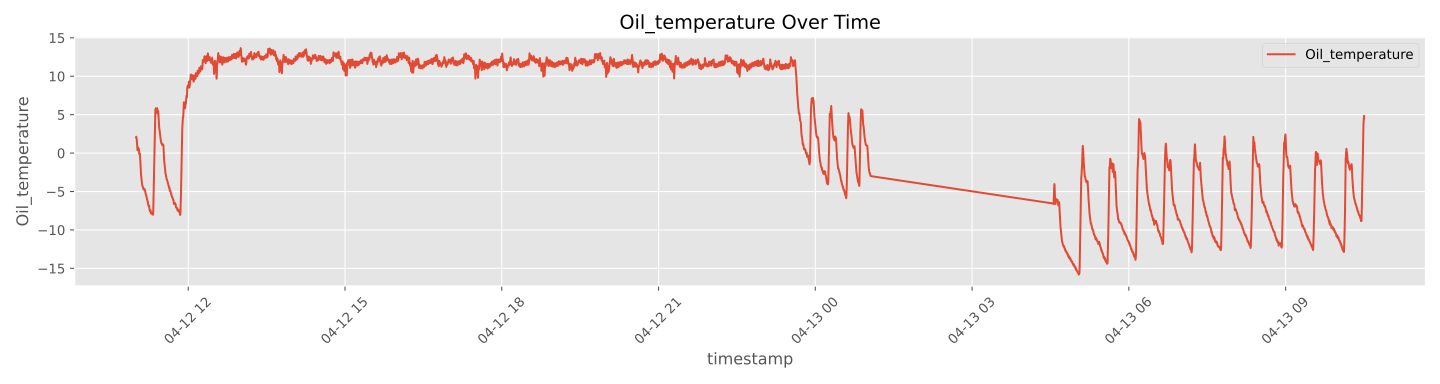
\includegraphics[width=\textwidth]{Oil_temperature.png}
        \caption*{Oil temperature}
    \end{minipage}
    \vspace{0.5em}
\caption{Variables en rangos donde hay anomalías. Se observa cambios bruscos en la naturaleza cíclica del uso habitual del motor de compresión.}
\label{fig:anomaly_in_variables}
\end{figure}

\begin{figure}[htp]
    \centering
    \begin{minipage}[b]{0.45\textwidth}
        \centering
        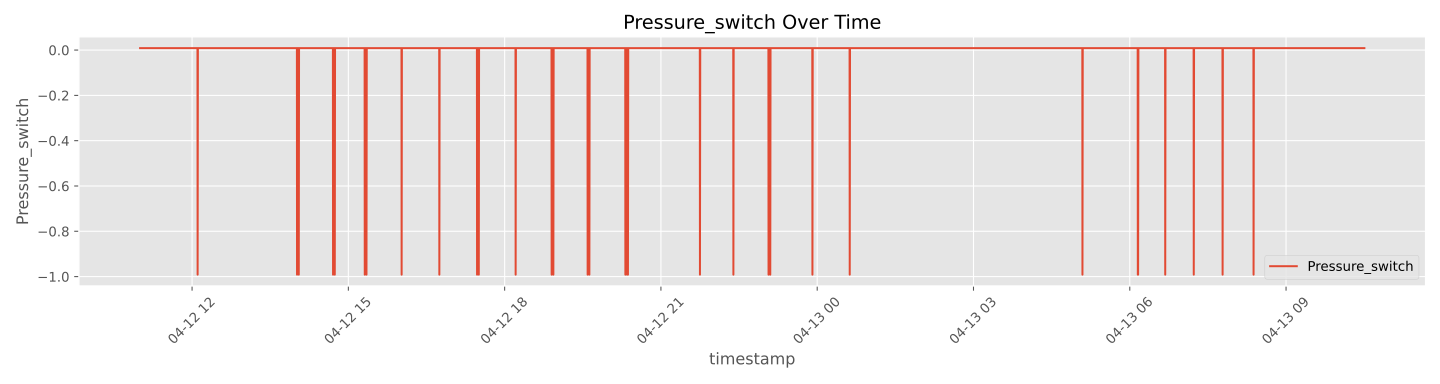
\includegraphics[width=\textwidth]{Pressure_switch.png}
        \caption*{Pressure switch}
    \end{minipage}
    \hfill
    \begin{minipage}[b]{0.45\textwidth}
        \centering
        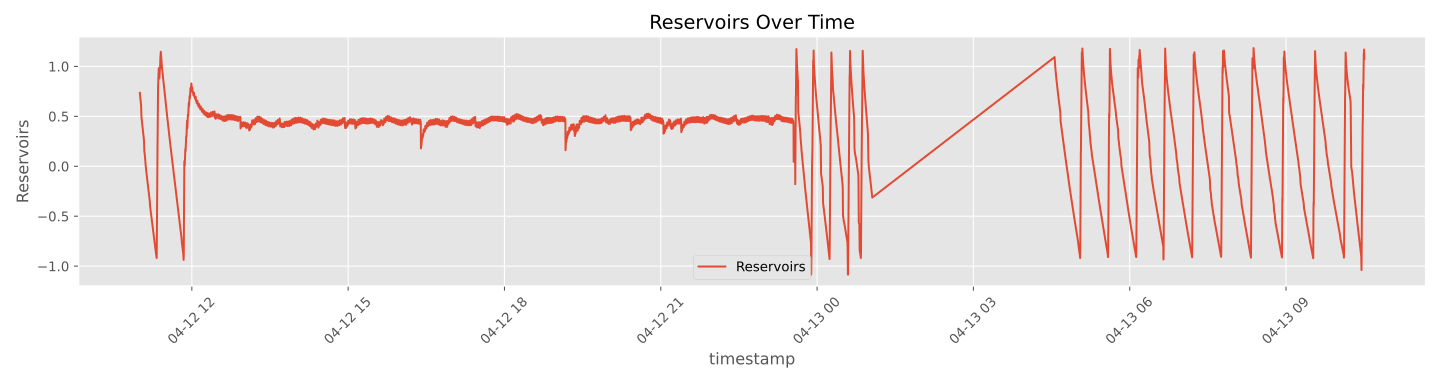
\includegraphics[width=\textwidth]{Reservoirs.png}
        \caption*{Reservoirs}
    \end{minipage}
    \vspace{0.5em}

    \begin{minipage}[b]{0.45\textwidth}
        \centering
        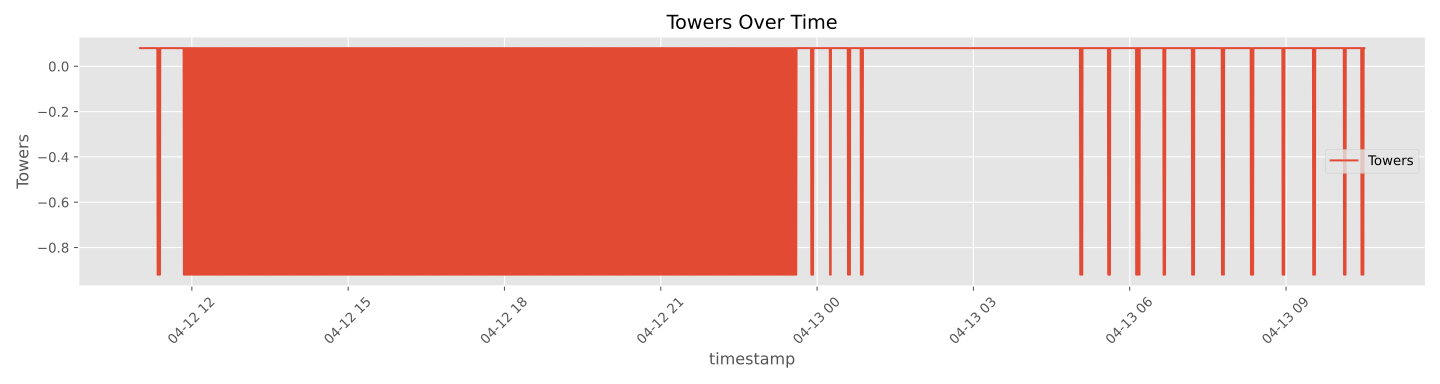
\includegraphics[width=\textwidth]{Towers.png}
        \caption*{Towers}
    \end{minipage}
    \hfill
    \begin{minipage}[b]{0.45\textwidth}
        \centering
        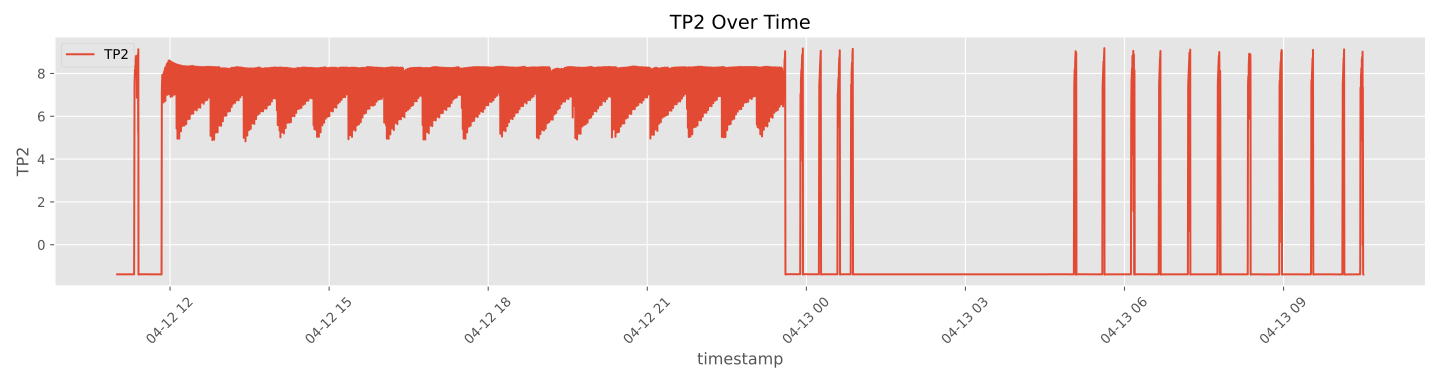
\includegraphics[width=\textwidth]{TP2.png}
        \caption*{TP2}
    \end{minipage}
    \vspace{0.5em}

    \begin{minipage}[b]{0.45\textwidth}
        \centering
        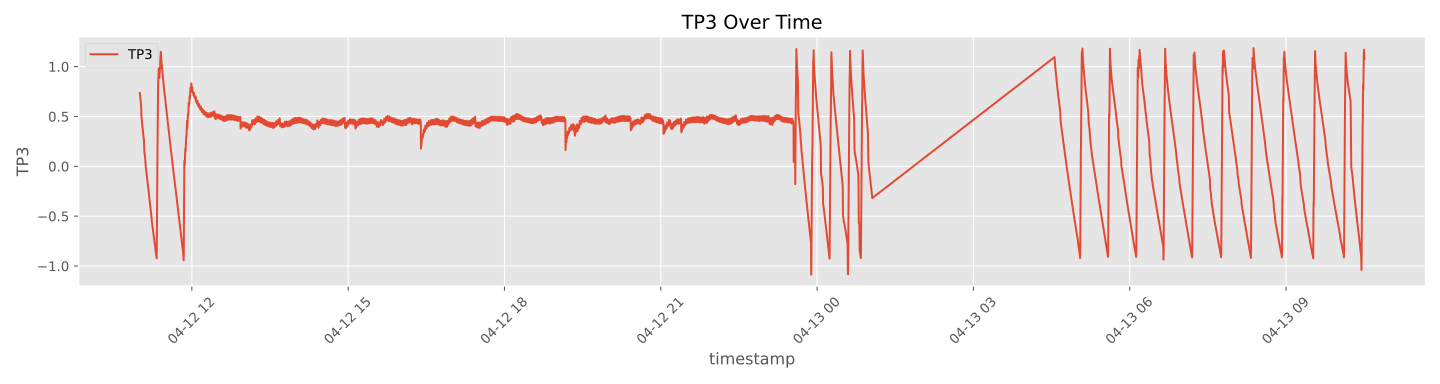
\includegraphics[width=\textwidth]{TP3.png}
        \caption*{TP3}
    \end{minipage}

    \caption{Variables en rangos donde hay anomalías.}
    \label{fig:anomaly_in_variables2}
\end{figure}

Como puede observarse en la Figura~\ref{fig:anomaly_in_variables} y en la Figura~\ref{fig:anomaly_in_variables2}, se visualizan los rangos donde según expertos, se produjo una anomalía. Gracias a esto es posible observar con facilidad que tipo de forma toma cada variable cuando una anomalía ocurre.

\begin{figure}[htp]
    \centering
    \subfloat{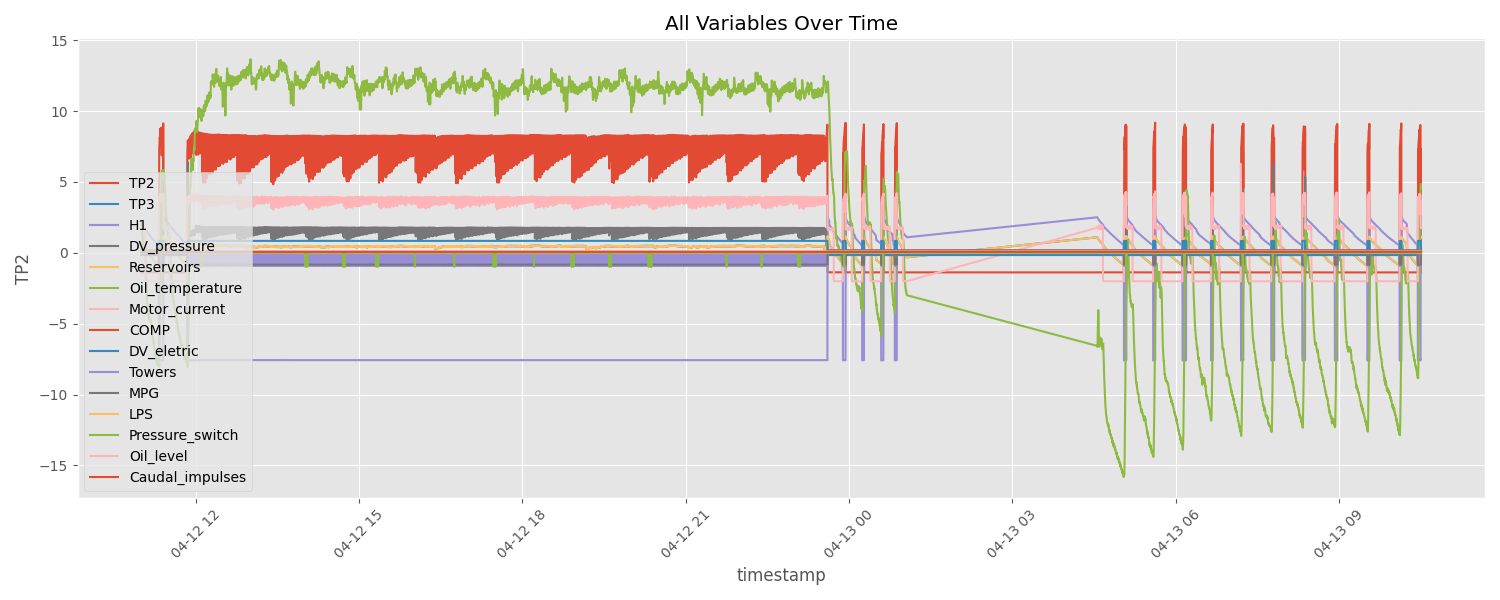
\includegraphics[width=0.7\textwidth]{all_anomalies.png}}
    \caption{Todas las variables en rango anómalos. Se observa la naturaleza cíclica de todas las variables debido a que iteraccionan en conjunto.}
    \label{fig:all_anomalies}
\end{figure}

En la Figura~\ref{fig:all_anomalies} se muestran todas las anomalías (centradas gracias al estandarizado sobre la media) y cómo se comportan en un rango anómalo. Se preserva la varianza de cada una de ellas de forma que pueda observarse su rango de valores completo real.

\begin{figure}[htp]
    \centering
    \subfloat{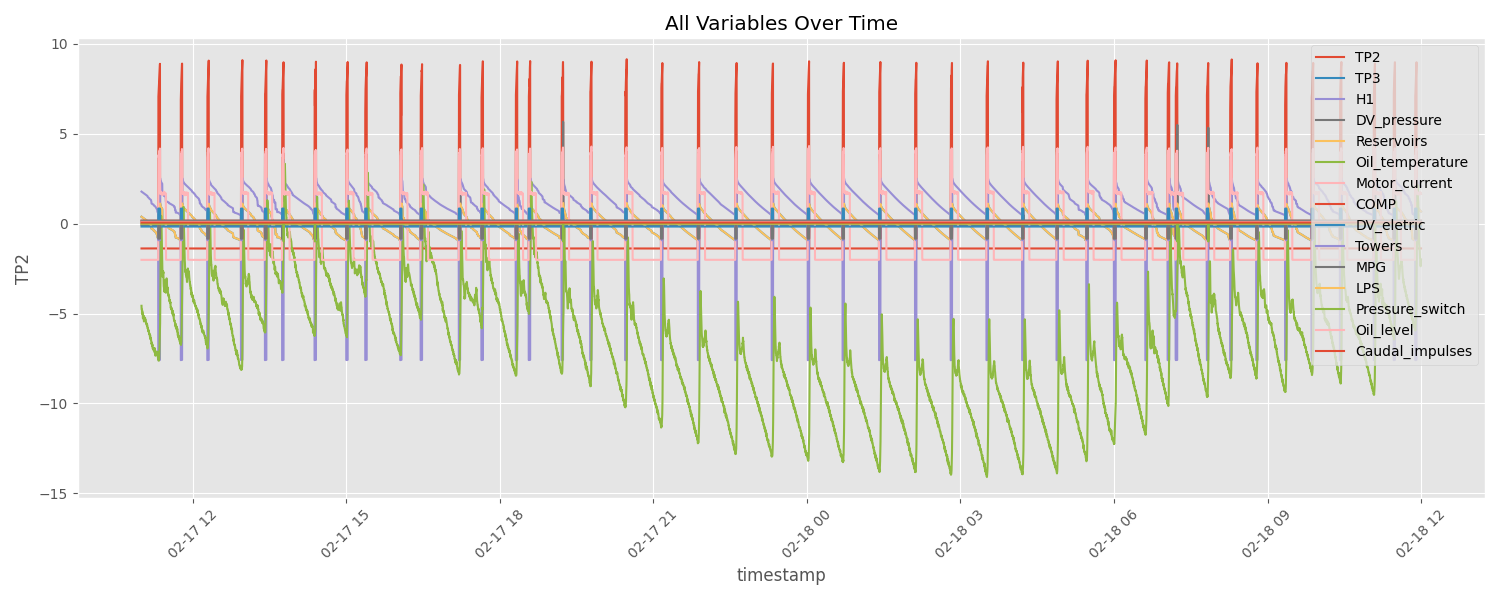
\includegraphics[width=0.7\textwidth]{all_normal.png}}
    \caption{Todas las variables en rangos normales.}
    \label{fig:all_normal}
\end{figure}


Si se muestra otro rango temporal, se puede observar el comportamiento esperado de cada variable. De hecho, se podría intuir que son series de naturaleza \textbf{estacionaria}. Este fenómeno puede observarse en la Figura~\ref{fig:all_normal}.
Una serie estacionaria es una secuencia de datos temporales cuyas propiedades estadísticas, como la media, la varianza y la autocorrelación, son constantes a lo largo del tiempo. Esto significa que su comportamiento no cambia dependiendo del momento en el que se analice, lo que facilita su modelado y predicción.

\subsection{Test estadísticos}
Se realizan pruebas estadísticas a las series temporales con el objetivo de determinar si son estacionarias. En este contexto, si el valor crítico de la prueba es mayor que el valor estadístico obtenido, se concluye que la serie no es estacionaria.
Entre las pruebas utilizadas, destaca la prueba de \textit{Dickey-Fuller Aumentada} (ADF), un test estadístico diseñado para evaluar la presencia de una raíz unitaria en una serie temporal. La existencia de una raíz unitaria indica que la serie no es estacionaria.

Ya que se tienen muchos datos, hacer la prueba de \textit{adfuller} con todos en cada columna no es viable. Por tanto, de manera aleatoria se escogen muestras de tramos aleatorios de cada variable. De esta manera se puede evaluar si la serie es estacionaria en gran parte de sus tramos y deducir si la serie completa es posible que sea estacionaria.

\begin{table}[htp]
    \centering
    \begin{tabular}{lcccc}
    \hline
    Variable & Repetitions & Avg. Test Stat & Avg. p-value & Stationary \\
    \hline
    TP3 & 9/10 & -5.32 & $10^{-4}$ & Yes \\
    H1 & 10/10 & -6.24 & $10^{-7}$ & Yes \\
    DV\_eletric & 8/10 & -5.68 & $10^{-6}$ & Yes \\
    DV\_pressure & 9/10 & -21.32 & $10^{-22}$ & Yes \\
    Caudal\_impulses & 0/10 & - & - & Constant \\
    TP2 & 9/10 & -6.29 & $10^{-7}$ & Yes \\
    Pressure\_switch & 9/10 & -20.91 & $10^{-13}$ & Yes \\
    Reservoirs & 10/10 & -5.68 & $10^{-6}$ & Yes \\
    Towers & 10/10 & -6.81 & $10^{-9}$ & Yes \\
    LPS & 1/10 & -4.76 & $10^{-5}$ & Partial \\
    Oil\_level & 2/10 & -2.59 & $0.1$ & No \\
    COMP & 10/10 & -5.99 & $10^{-6}$ & Yes \\
    Motor\_current & 9/10 & -4.56 & $10^{-4}$ & Yes \\
    MPG & 9/10 & -6.09 & $10^{-7}$ & Yes \\
    Oil\_temperature & 10/10 & -5.28 & $10^{-5}$ & Yes \\
    \hline
    \end{tabular}
    \caption{Tabla de resultados tras $10$ repeticiones en tramos aleatorios}
    \label{tab:stationary_results}
\end{table}

Como puede verse en la Tabla~\ref{tab:stationary_results}.

\subsection{Preprocesamiento}

\subsubsection{Enfoques del problema}


Existen dos enfoques principales para abordar el estudio de este problema, los cuales varían dependiendo de si se incorporan o no valores temporales. El \textbf{primer enfoque} se basa en el uso de \textbf{instantáneas} y prescinde de la información temporal. En este enfoque, en cada iteración, los sensores del compresor generan un vector de valores representativos del estado del sistema en ese momento específico. Este vector se puede utilizar para predecir la presencia de posibles anomalías en el compresor, sin considerar las variaciones temporales previas.

Este método tiene la ventaja de permitir una detección rápida de anomalías, ya que, si es capaz de identificar correctamente los fallos, proporcionaría una respuesta con el menor retardo posible, e incluso en tiempo real. La ventaja principal de este enfoque radica en su simplicidad y capacidad de ofrecer una alerta inmediata ante cualquier fallo en el compresor, lo que resulta crucial en aplicaciones donde la rapidez en la respuesta es fundamental.

El \textbf{segundo enfoque} se basa en la \textbf{incorporación de información temporal} y utiliza valores dentro de una ventana de tiempo determinada para identificar posibles fallos en el compresor. A través de este enfoque, el modelo encargado de la detección de anomalías es capaz de realizar un análisis más detallado de las tendencias a lo largo del tiempo. Este análisis temporal permite captar patrones que, de otro modo, podrían pasar desapercibidos al considerar únicamente instantáneas.

Es razonable suponer que ciertos fallos no se manifiestan mediante cambios abruptos en los valores de los sensores, sino que se desarrollan progresivamente. Por ejemplo, una disminución gradual del nivel de aceite, que ocurre a una velocidad mayor de la esperada, podría ser suficiente para señalar el inicio de un fallo. En estos casos, el análisis de los valores temporales sería esencial, ya que permite detectar anomalías antes de que los valores de los sensores alcancen niveles extremos. Esto, en un contexto predictivo, posibilitaría adelantarse al fallo y, potencialmente, evitarlo.

No obstante, este enfoque no está exento de desafíos. Una de las principales limitaciones es que los valores anómalos pueden quedar ``opacados'' o diluidos por el resto de los datos dentro de la ventana temporal, lo que podría dificultar la identificación precisa de anomalías. Sin embargo, el equipo considera que la información temporal ofrece una ventaja significativa en la detección temprana de fallos, por lo que ha decidido centrar su trabajo en este enfoque. A continuación, se abordarán con mayor detalle las características de este modelo y cómo se gestionan los posibles problemas derivados de la utilización de información temporal en el proceso de detección.

\subsubsection{Definición de la ventana deslizante}

Para resolver este problema estudiamos los tiempos de activaciones de los motores para poder definir una ventana deslizante que pueda recoger información de la activación de los mismos. 
Para ello, se ha calculado la mediana del tiempo de activación de los motores. Para ello, se ha detectado la activación y apagado del motor por medio de la variable ``Motor\_current'', cuyos 
valores para apagado son inferiores a 0.05, veáse la Figura~\ref{fig:VisualizacionDatos}.

\begin{figure}[htp]
        \centering
        \subfloat{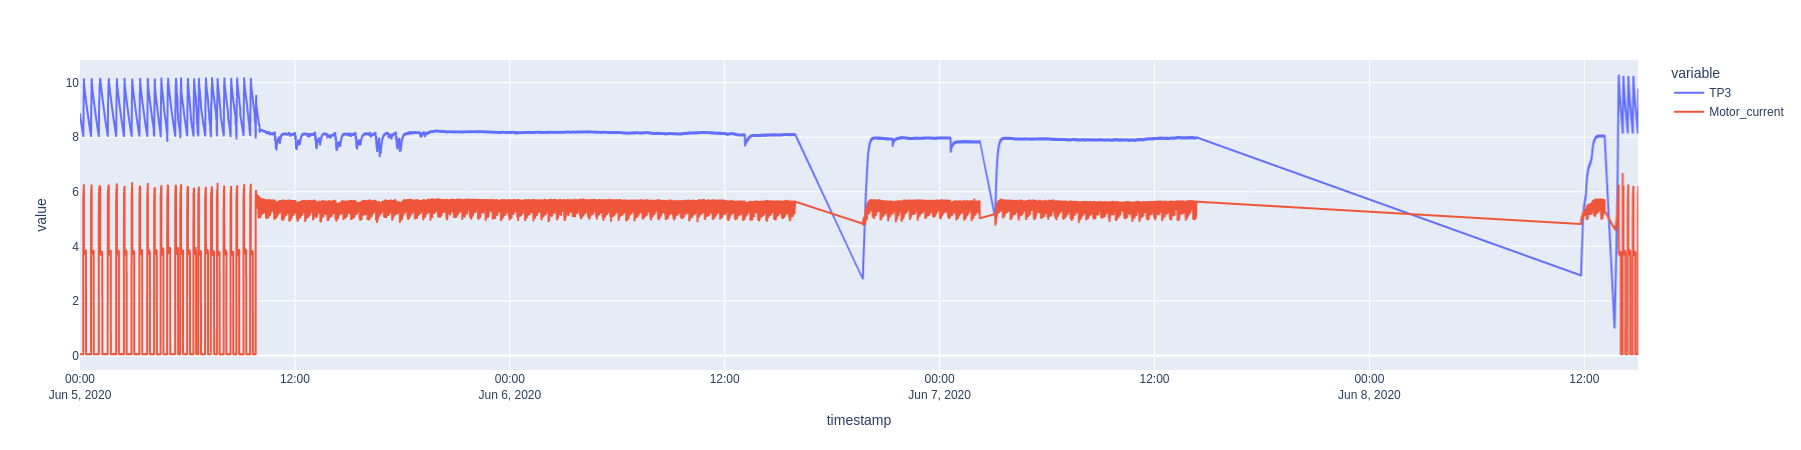
\includegraphics[width=0.7\textwidth]{VisualizacionDatos.png}}
        \caption{Observamos los datos y los valores de la presión en el panel neumático (TP3, línea azul) y la corriente del motor (línea roja).}
        \label{fig:VisualizacionDatos}
\end{figure}

Se han recogido los resultados en la Tabla~\ref{tab:TiempoCiclo}. La mediana se calcula sobre los intervalos de tiempo no anómalos. No obstante, 
aunque el conjunto de datos no presenta valores pérdidos en ninguna de las columnas, sí que presenta saltos temporales. Los datos de los sensores se mostrean cada 10 segundos, 
pero se ha encontrado saltos temporales de incluso días, véase Figura~\ref{fig:VentanaDeslizante}. Se planteó la posibilidad de interpolar los datos, pero dada la naturaleza 
del problema, serie temporal pseudo-cíclica pero con intervalos distintos, es difícil obtener resultados prometedores para saltos grandes sin la posibilidad de ``ensuciar'' la calidad de los datos.
Por ello, se ha calculado el tiempo mediano de ciclo de motor tras eliminar los saltos temporales. Para comprobar, se ha calculado también la mediana 
para todos intervalos sin anomalías de la Tabla~\ref{tab:Reportes}. Los valores obtenidos están muy cerca del especificado en la Tabla~\ref{tab:TiempoCiclo}.

\begin{table}[htp]
    \centering
    \begin{tabular}{|c|}
    \hline
    \textbf{Mediana del tiempo de ciclo} \\ \hline 
    1260 segundos\\
    \hline
    \end{tabular}
    \caption{Resultado obtenido del cálculo de la ventana deslizante. Se acerca a los obtenidos en el artículo original de detección de fallos de este dataset~\cite{FailureDetection}.}
    \label{tab:TiempoCiclo}
\end{table}

Para la asignación de los grupos se ha utilizado dos veces la mediana del tiempo de ciclo del motor. 
Esto es debido a que así se puede asegurar contener información de almenos más de la mitad de la activación del motor, asegurando que predecimos con la mayor información posible del estado del motor.
Se puede observar la asignación de grupos en la Figura~\ref{fig:VentanaDeslizante}.

\begin{figure}[htp]
        \centering
        \subfloat{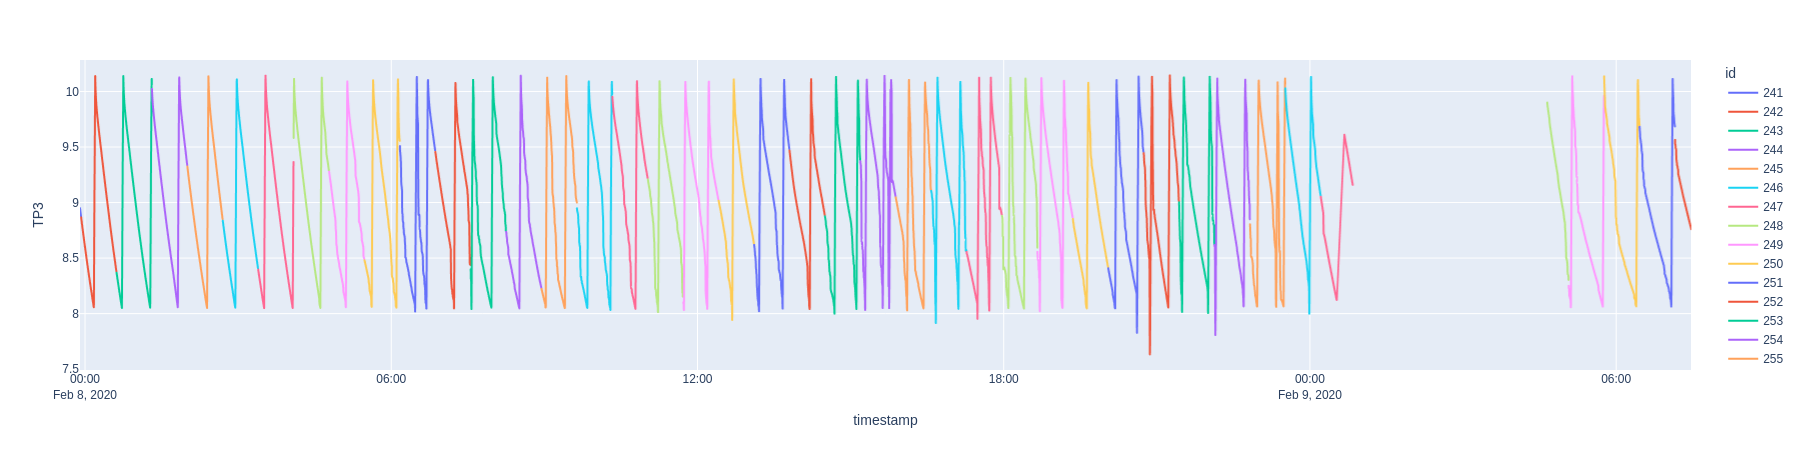
\includegraphics[width=0.7\textwidth]{VentanaDeslizante.png}}
        \caption{Observamos los grupos asignados de utilizar 2 veces el tiempo de ciclo.}
        \label{fig:VentanaDeslizante}
\end{figure}


Durante el análisis EDA y prepración del conjunto de datos de entrenamiento y evaluación se han recogido nuevas anomalías, veáse la Tabla~\ref{tab:EventosRaros} y Figura~\ref{fig:EventosRaros}.
Sería interesante volver a consultar con un experto del campo para que valide dichas anomalías. No obstante, presentan un perfil suficientemente cercano al de las anomalías clasificadas.
Por ello, consideramos oportuno la inclusión de dichos ejemplos como anomalías para ayudar a resolver el problema del bajo número de ejemplo de casos positivos.

\begin{table}[htp]
    \centering
    \begin{tabular}{|c|l|l|r|l|}
    \hline
    \textbf{Número} & \textbf{Inicio}       & \textbf{Fin}         & \textbf{Duración (min)} & \textbf{Importancia} \\ \hline
    22 & 2020-03-06 21:42:15 & 2020-03-06 23:14:00 & 92 & - \\ \hline
    23 & 2020-03-11 05:15:10 & 2020-03-11 06:25:00 & 70 & - \\ \hline
    24 & 2020-03-12 00:15:56 & 2020-03-12 11:59:00 & 704 & - \\ \hline
    25 & 2020-03-26 04:00:20 & 2020-03-26 05:20:00 & 80 & - \\ \hline
    26 & 2020-03-27 07:12:00 & 2020-03-27 12:01:00 & 289 & - \\ \hline
    27 & 2020-04-17 08:50:28 & 2020-04-17 23:59:00 & 909 & - \\ \hline
    28 & 2020-04-25 00:07:15 & 2020-04-25 01:10:00 & 63 & - \\ \hline
    29 & 2020-05-19 01:35:28 & 2020-05-19 02:40:00 & 64 & - \\ \hline
    30 & 2020-06-12 01:41:07 & 2020-06-12 17:06:00 & 925 & - \\ \hline
    31 & 2020-07-21 13:32:48 & 2020-07-21 22:03:00 & 510 & - \\ \hline
    32 & 2020-07-22 06:40:46 & 2020-07-22 13:10:00 & 389 & - \\ \hline
    33 & 2020-07-31 00:57:33 & 2020-07-31 02:09:00 & 71 & - \\ \hline
    \end{tabular}
    \caption{Intervalos de tiempo encontrados con valores constantes y fluctuaciones extrañas, un patrón similar al de las anomalías, sin etiquetado.}
    \label{tab:EventosRaros}
\end{table}

\begin{figure}[htp]
        \centering
        \subfloat{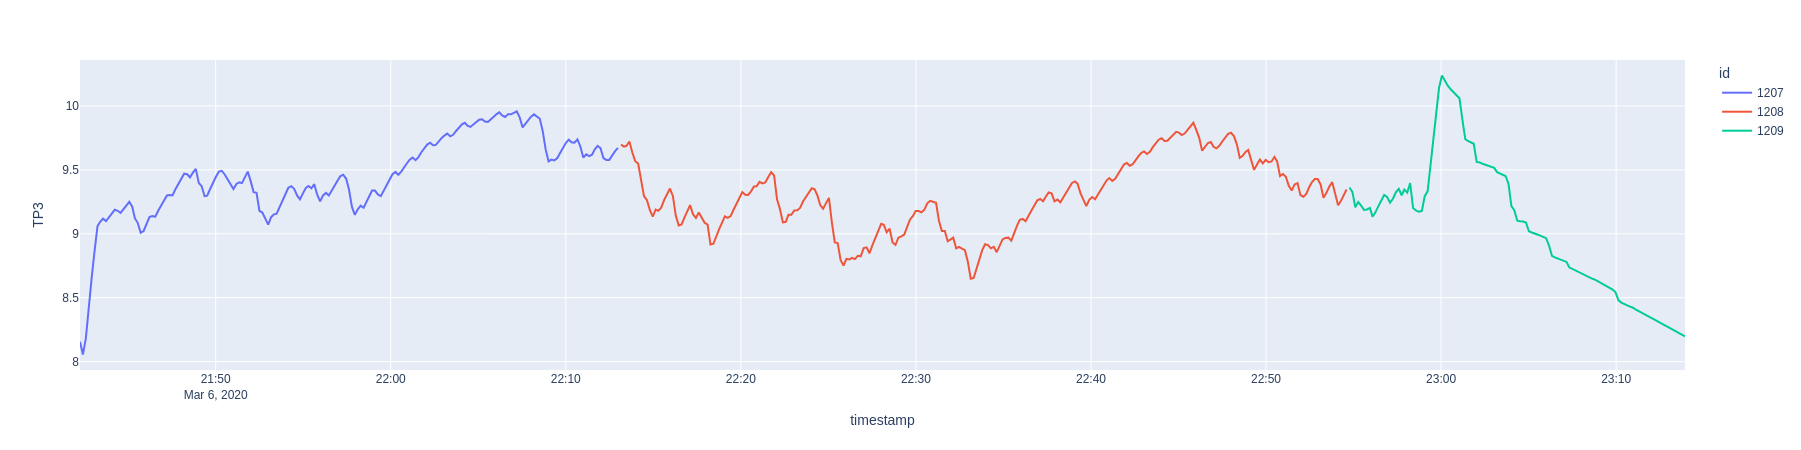
\includegraphics[width=0.7\textwidth]{EjemploRaro1.png}}\\
        \subfloat{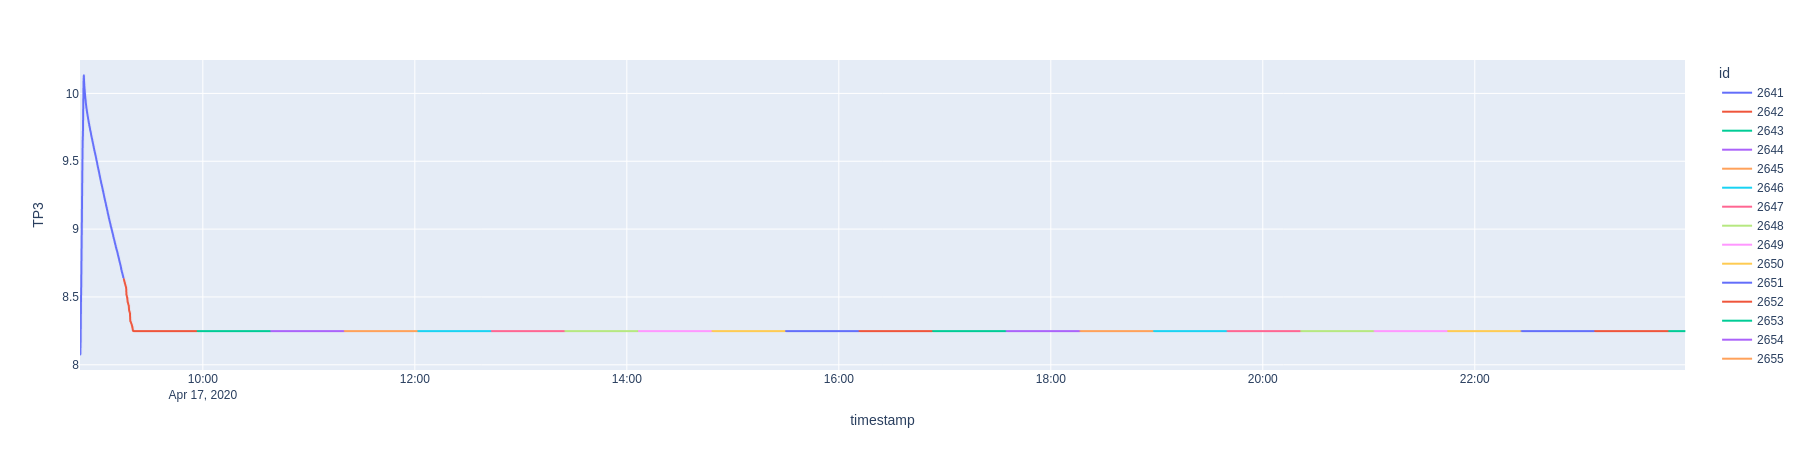
\includegraphics[width=0.7\textwidth]{EjemploRaro2.png}}
        \caption{Ejemplo de nuevos intervalos anómalos encontrados. Observamos valores constantes o fluctuaciones fuera de lo habitual para el motor apagado o encendido.}
        \label{fig:EventosRaros}
\end{figure}

Tras observar y analizar el conjunto de datos, seguimos un acercamiento similar a~\cite{PredictiveMaintenance,FailureDetection} para tratar a la serie temporal, 
se ha optado por la transformación de los intervalos de las ventanas deslizante en obtener el promedio, mínimo, máximo y varianza de cada variable durante el intervalo de tiempo mostreado. 
Para resolver el problema de saltos temporales, se ha eliminado aquellos conjuntos en los que se estiman estas variables para un número de puntos inferior a $(\textrm{tiempo de ciclo}) / 10 = 126$. Ya que esos ejemplos 
son estimados con menos puntos que el tiempo de activación del motor, lo cuál puede generar estimaciones del promedio y varianza sub-óptimos.

\subsubsection{Generación de conjuntos}

Una vez determinado la ventana deslizante y las características a extraer, se genera las diferentes instancias y se divide en los conjuntos de entrenamiento y evaluación. Se debe determinar por tanto si un intervalo de la ventana deslizante es una anomalía o no, para lo cuál es utilizado se utilizado un criterio de votación en el cuál gana la mayoría.

Uno de los aspectos cruciales a considerar en este enfoque es la similitud de los datos generada por la ventana deslizante en ciertos momentos. Por ejemplo, en el caso de anomalías cuya duración se extiende por un periodo de tiempo considerable, como un día completo (por ejemplo, de 6/05/2020 10:00 a 6/05/2020 23:59), se generan ventanas de 21 minutos en cada iteración. Esto puede dar lugar a la aparición de instantes temporalmente muy similares entre sí, lo que podría influir en la evaluación de los modelos de detección de anomalías.

Una situación problemática podría ocurrir si las ventanas se distribuyeran de manera completamente aleatoria a posteriori. En ese caso, se podría dar el escenario en el cual un periodo como \textbf{6/05/2020 10:00 - 6/05/2020 10:21} pertenezca al conjunto de entrenamiento, mientras que el siguiente periodo \textbf{6/05/2020 10:21 - 6/05/2020 10:42} esté en el conjunto de test. Esta división podría generar evaluaciones poco representativas, ya que las ventanas de tiempo consecutivas podrían estar separadas en diferentes conjuntos de datos, lo que afectaría la validez de la evaluación de la capacidad predictiva del modelo. Véase la figura \ref{fig:VentanaDeslizante}.

\begin{figure}[htp]
        \centering
        \subfloat{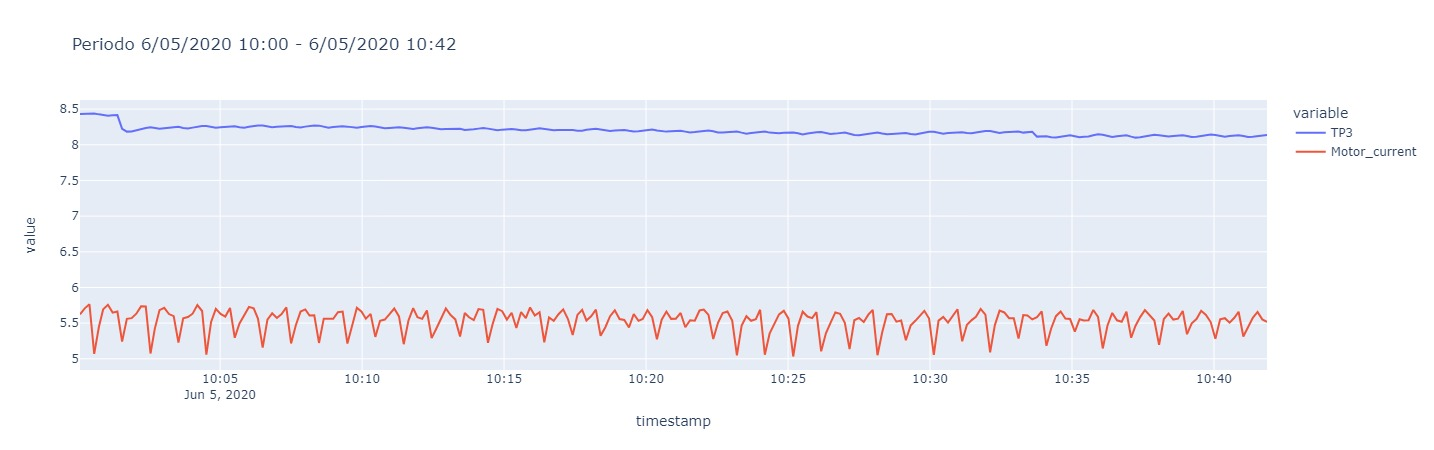
\includegraphics[width=0.7\textwidth]{prueba_agrupacion.jpeg}}
        \caption{Observamos la similitud de los valores de algunos sensores durante la anomalía.}
        \label{fig:PruebaAgrupacion}
\end{figure}

Para mitigar este riesgo y garantizar una evaluación más precisa y coherente, las instancias se agrupan temporalmente. De esta forma, se asegura que dos instancias pertenecientes al mismo grupo no se distribuyan entre los conjuntos de entrenamiento y test si dichos conjuntos se utilizan con fines de validación y entrenamiento. Se define un \textbf{grupo} como un conjunto de ventanas que comparten el mismo tipo (anomalía o no anomalía) y no presentan saltos temporales, es decir, no existe un periodo sin datos entre las ventanas. Este enfoque asegura que la información utilizada en el entrenamiento y la validación sea coherente y representativa, mejorando así la robustez de las evaluaciones del modelo.

El proceso de generación de los conjuntos de datos consiste en barajar los grupos de ventanas deslizantes para asignar de forma aleatoria diferentes grupos de intervalos de tiempo en cada partición, 
evitando así pliegues más fáciles o difíciles (obtener unos resultados más balanceados en general). Es decir, agrupamos los grupos en grupos de mayor tamaño, pero esta vez mediante la aleatoriedad y teniendo en cuanta la proporción de grupos anómalos y grupos no anómalos.

Concretamente, se decide dividir los datos en 9 pliegues. Se estima el número de anomalías que pertenecería a cada pliegue y se genera conjuntos lo más equilibrado posible (véase la Tabla~\ref{tab:ValidacionCruzada}). 
Por último, se asigna el pliegue 1 y 8 (elección aleatoria) como el conjunto de test. Los resultantes serán agrupado en 4 pliegues para el entrenamiento de la validación cruzada. 

\begin{table}[htp]
    \centering
    \begin{tabular}{|c|c|c|c|}
    \hline
    \textbf{Pliegue} & \textbf{Negativo} & \textbf{Positivo} & \textbf{Conjunto}\\ \hline
    0 & 635 & 31 & Evaluación \\ \hline
    1 & 635 & 31 & Etrenamiento pliegue 1 \\ \hline
    2 & 635 & 31 & Etrenamiento pliegue 2\\ \hline
        3 & 635 & 31 & Etrenamiento pliegue 3\\ \hline
        4 & 635 & 31 & Etrenamiento pliegue 4\\ \hline
        5 & 635 & 31 & Etrenamiento pliegue 3\\ \hline
        6 & 635 & 31 & Etrenamiento pliegue 2 \\ \hline
        7 & 638 & 31 & Etrenamiento pliegue 1\\ \hline
        8 & 641 & 43 & Evaluación \\ \hline
    \end{tabular}
    \caption{Distribución de los 9 pliegues generados. Se asigna de forma aleatoria el 1 y 8 a test. Se agrupan los demás hasta forma 4 pliegues usando el primer y último de los restantes: 0 y 7, 2 y 6, 5 y 3, 4.}
    \label{tab:ValidacionCruzada}
\end{table}

\section{Regresión Logística.}
\section{Máquinas de Vectores de Soporte.}
\section{Clasificador Bayesiano.}
\section{Árboles de clasificación.}
\section{Gradient Boosting.}
\section{Stacking.}
\section{AdaBoost.}
\section{Bagging.}
\printbibliography
\end{document}
